\section{"1" Определение геометрических свойств поверхности}

\begin{frame}[t]{Определение геометрических свойств}
\framesubtitle{}
    \begin{columns}[T,onlytextwidth]
        \begin{column}{0.69\textwidth}
            \small
            С помощью \textbf{ощупывания роботом поверхности} получить \underline{плотное облако точек} и \underline{полигональную сетку}.

            \textbf{Метод решения}: Триангуляция Делоне с использованием альфа формы

            \textbf{Алгоритм}: Решив задачу локализации, получить облако точек следовой дорожки. \textbf{Очистить шумное облако точек} и его \textbf{усреднить} с помощью Voxel Grid. Применить \underline{триангуляцию Делоне для вогнутых оболочек}, получив полигональную сетку. \underline{Сгенерировать новые точки} из полигональной сетки с нужным разрешением.

            \textbf{Входные данные}: следовая дорожка, в виде облака точек.
            
            \textbf{Выходные данные}: полигональная сетка и плотное облако точек
            
            \textbf{Допустимая точность}: 0.1 м, оценки Cloud2Cloud и Cloud2Mesh

            \textbf{Предположения}: 1) Имеется поверхность. Координаты задаются $z=f(x,y)$. 2) Расстояние между ногами робота мало относительно размеров поверхности, следовательно, поверхность между ногами считается плоскостью.   
        \end{column}
        \begin{column}{0.29\textwidth}
            \begin{figure}[H]
                \begin{subfigure}{0.99\textwidth}
                    \centering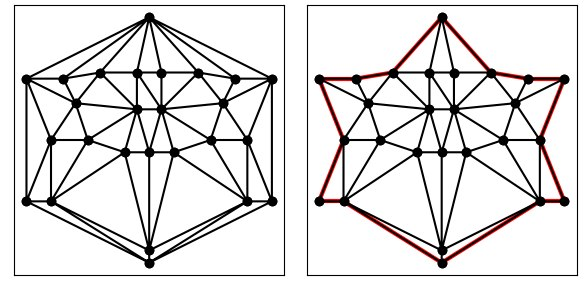
\includegraphics[height=2.5cm,width=1\textwidth,keepaspectratio]{../images/slides/delone_mag.png}
                    \caption*{Триангуляция Делоне}
                \end{subfigure}

                \begin{subfigure}{0.99\textwidth}
                    \centering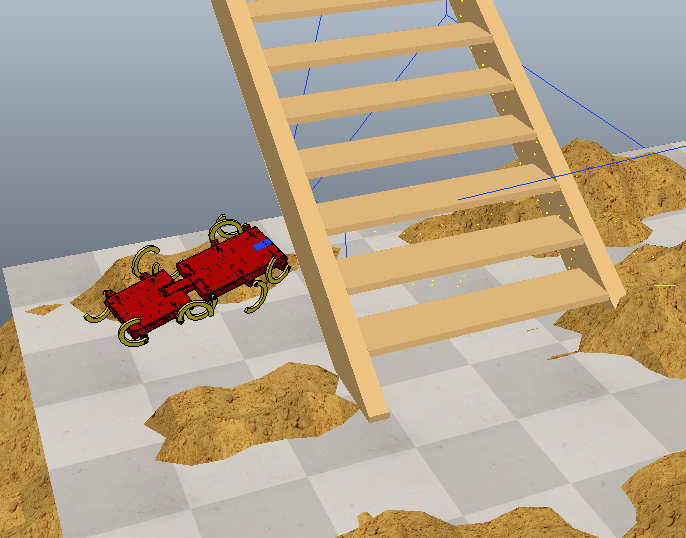
\includegraphics[height=2.5cm,width=1\textwidth,keepaspectratio]{../images/slides/error.png}
                    \caption*{Когда $z\neq f(x,y)$}
                \end{subfigure}
            \end{figure}
        \end{column}
    \end{columns}
\end{frame}

\note{Последняя задача, которая была решена - определение геометрических свойств пройденной поверхности. Необходимо с помощью ощупывания роботом поверхности получить плотное облако точек и полигональную сетку.}

\begin{frame}[t]{Оценки C2C и C2M}
\framesubtitle{}
    \begin{figure}[H]
        \begin{subfigure}[t]{0.49\textwidth}
            \centering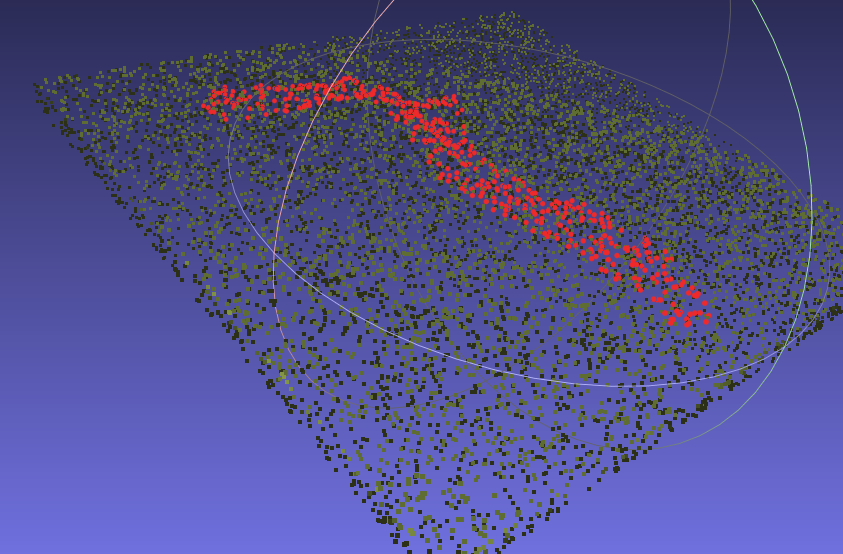
\includegraphics[height=4.5cm,width=1\textwidth,keepaspectratio]{../images/slides/c2c.png}
            \caption*{Cloud to Cloud: высчитывается абсолютное расстояние до ближайшей соседней точки}
        \end{subfigure}
        \begin{subfigure}[t]{0.49\textwidth}
            \centering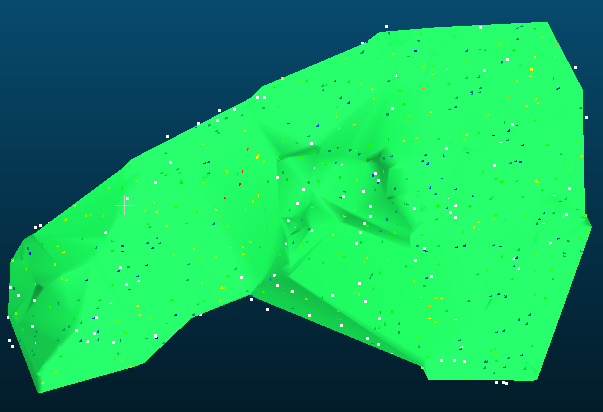
\includegraphics[height=4.5cm,width=1\textwidth,keepaspectratio]{../images/slides/c2m.png}
            \caption*{Cloud to Mesh: высчитывается расстояние с учетом знания о векторе нормали плоскости}
        \end{subfigure}
    \end{figure}
\end{frame}

\note{2}

\begin{frame}[t]{Эксперименты}
    \begin{figure}[H]
        \begin{subfigure}[t]{0.49\textwidth}
            \centering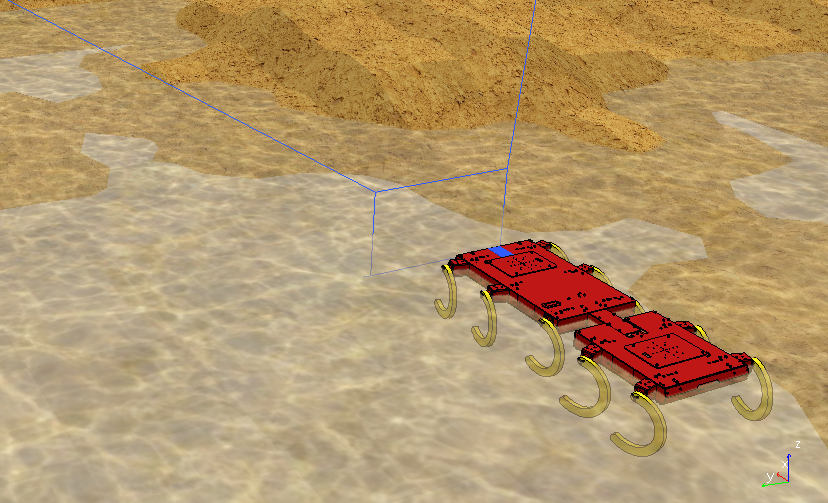
\includegraphics[height=5cm,width=1\textwidth,keepaspectratio]{coppelia_sim.png}
            \caption*{CoppeliaSim симулятор,\\ \textbf{4е поколение} СтриРус}
        \end{subfigure}
        \begin{subfigure}[t]{0.49\textwidth}
            \centering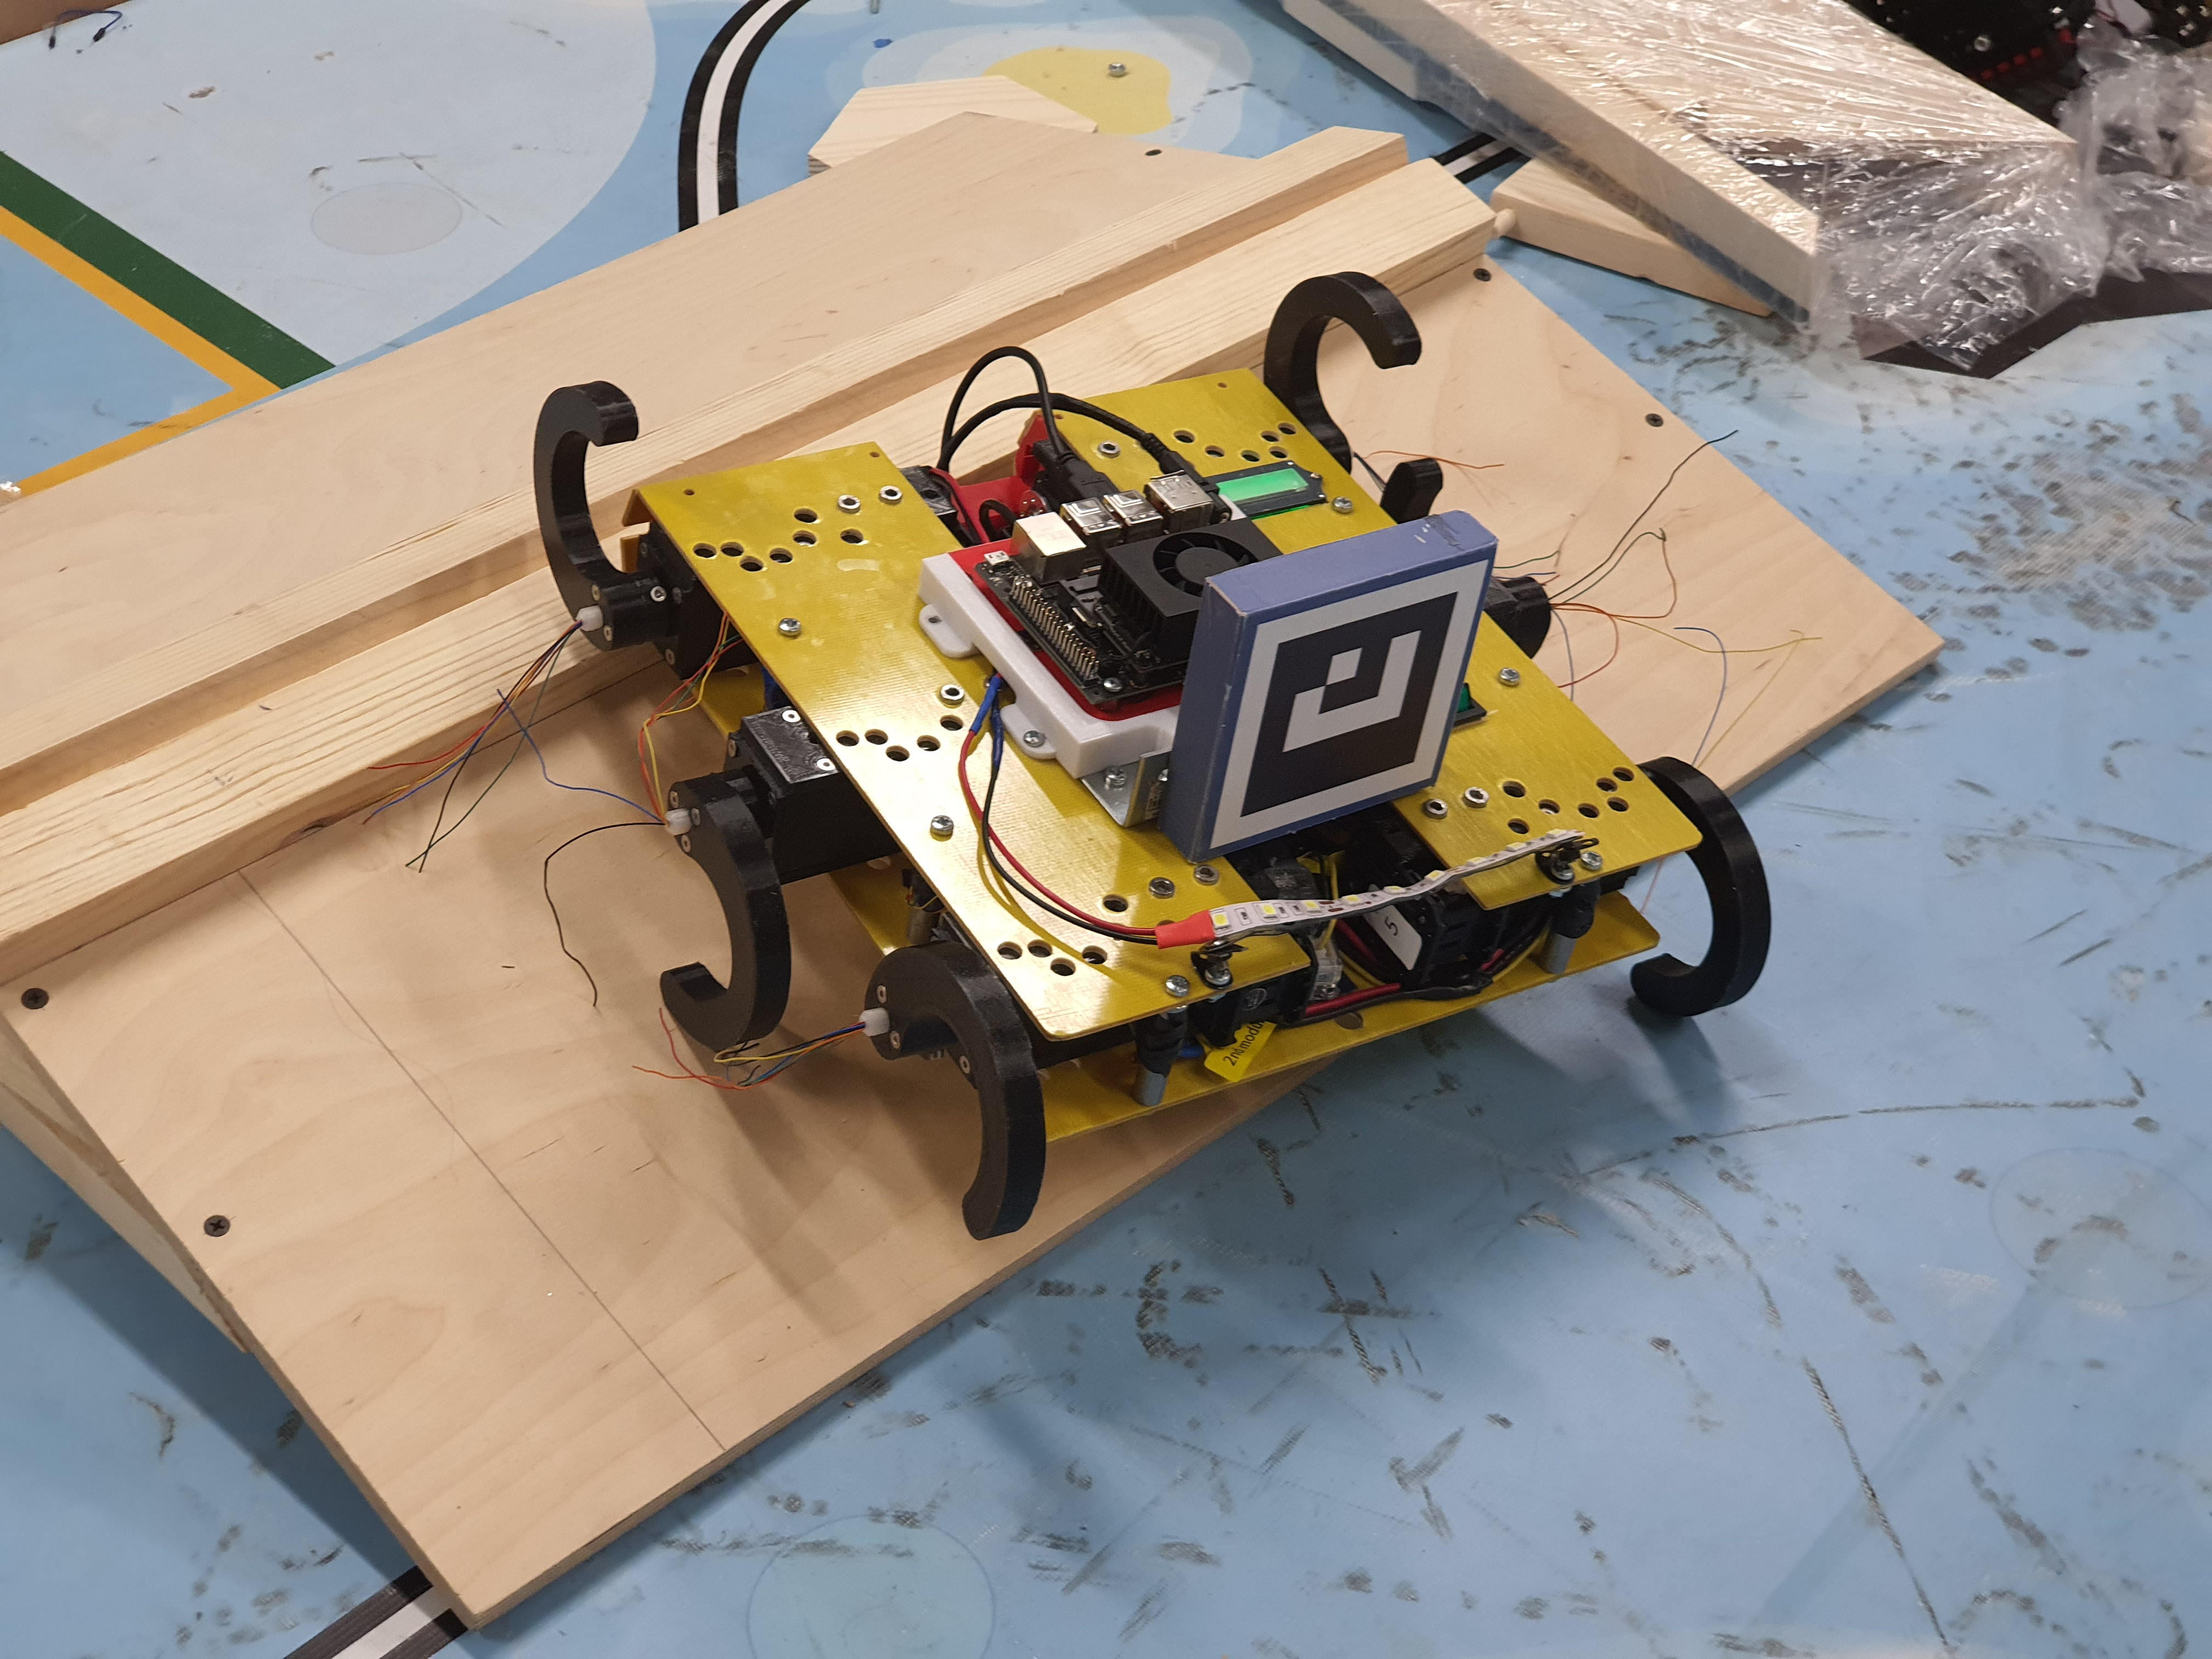
\includegraphics[height=5cm,width=1\textwidth,keepaspectratio]{rl_sim.JPG}
            \caption*{Натурные испытания,\\ \textbf{3е+ поколение} СтриРус}
        \end{subfigure}
    \end{figure}
\end{frame}

\note{a}

\begin{frame}[t]{Задача локализации}
\framesubtitle{}
\begin{multline}
        H_{leg}^{glob} = H(x_{glob},y_{glob},z_{glob},\alpha_{glob},\beta_{glob},\gamma_{glob})T_z(l_1)T_x(l_2)R_y(\alpha_3)T_x(l_4)T_y(l_5)R_z(-15^{\circ})T_y(l_7)R_y(\alpha_8)
\end{multline}

\vspace{-0.3cm}
Где $H = \begin{bmatrix}
    \underset{3 \times 3}{R} & \underset{3 \times 1}{T} \\
    \underset{1 \times 3}{0} & \underset{1 \times 1}{1}
\end{bmatrix}$, $R_i$ --- матрица поворота, относительно одной из осей, $T_i$ --- вектор сдвига.

    \begin{columns}[T,onlytextwidth]
        \begin{column}{0.69\textwidth}
            
            \vspace{-0.3cm}
            \begin{figure}[H]
        \centering
        \centering\includegraphics[height=4.5cm,width=1\textwidth,keepaspectratio,page=8]{./tikz_pictures.pdf}
    \end{figure}
        \end{column}
        \begin{column}{0.29\textwidth}
            \begin{figure}[H]
                \centering\includegraphics[height=6cm,width=1\textwidth,keepaspectratio]{../images/slides/snow_local.png}
                \caption{Пример решения задачи локализации с помощью Aruco маркера}
            \end{figure}
        \end{column}
    \end{columns}
\end{frame}

\note{mm}

\begin{frame}[t]{Делоне для вогнутых оболочек}
    \begin{figure}[H]
        \begin{subfigure}[t]{0.3\textwidth}
            \centering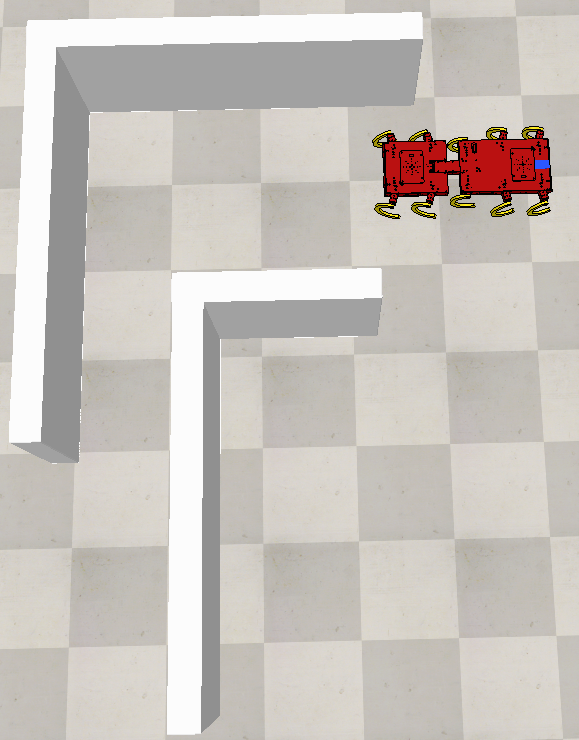
\includegraphics[height=5cm,width=1\textwidth,keepaspectratio]{convex_terr.png}
            \caption*{Пример поверхности}
        \end{subfigure}
        \hfill
        \begin{subfigure}[t]{0.33\textwidth}
            \centering
            \centering\includegraphics[height=6cm,width=1\textwidth,keepaspectratio,page=9]{./tikz_pictures.pdf}
            \caption*{Выпуклая оболочка}
        \end{subfigure}
        \hfill
        \begin{subfigure}[t]{0.33\textwidth}
            \centering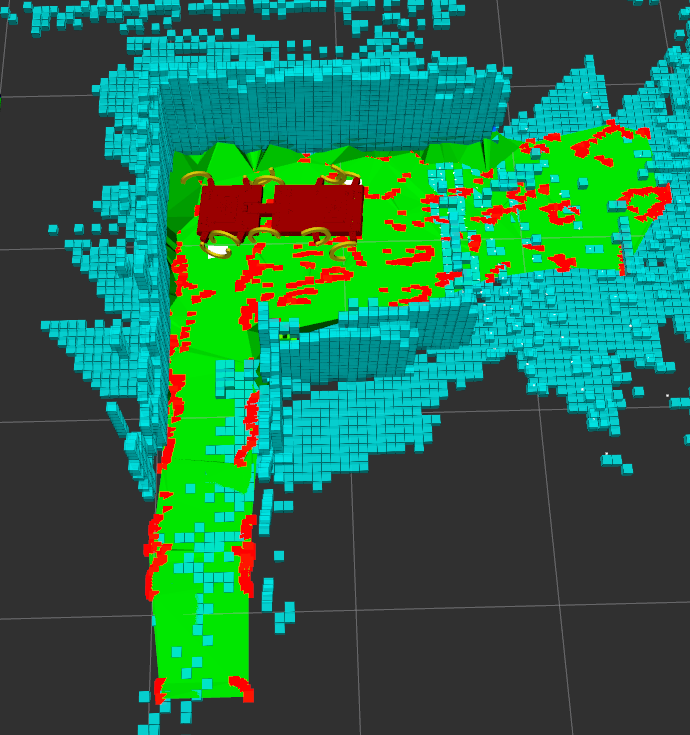
\includegraphics[height=6cm,width=1\textwidth,keepaspectratio]{conv_concave.png}
            \caption*{Вогнутая оболочка}
        \end{subfigure}

    \end{figure}
\end{frame}

\note{a}

\begin{frame}[t]{Определение геометрических свойств поверхности}
    \framesubtitle{Результат: Маршрут, полигональная сетка}
    \begin{figure}[H]
        \begin{subfigure}[t]{0.36\textwidth}
            \centering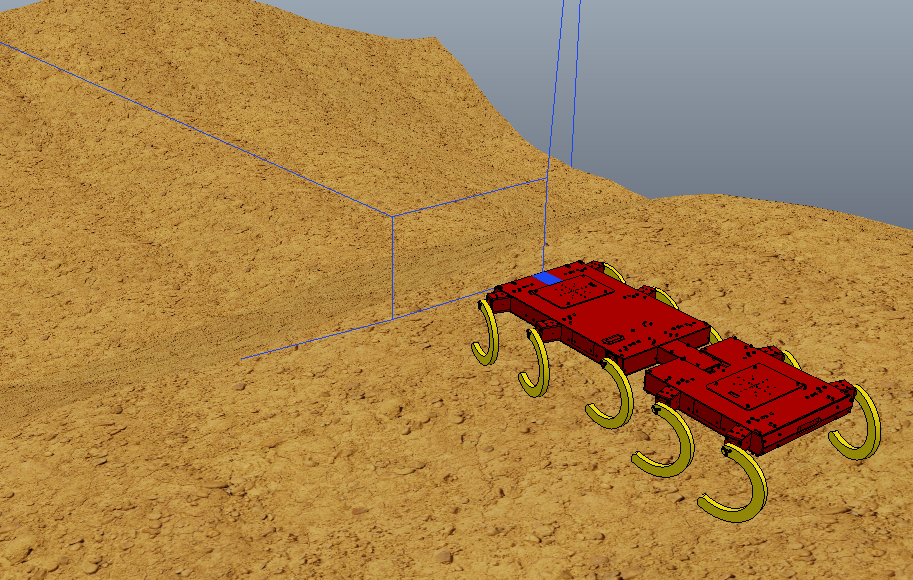
\includegraphics[height=5cm,width=1\textwidth,keepaspectratio]{terrain_wo_water.png}
            \caption*{Начало маршрута}
        \end{subfigure}
        \begin{subfigure}[t]{0.36\textwidth}
            \centering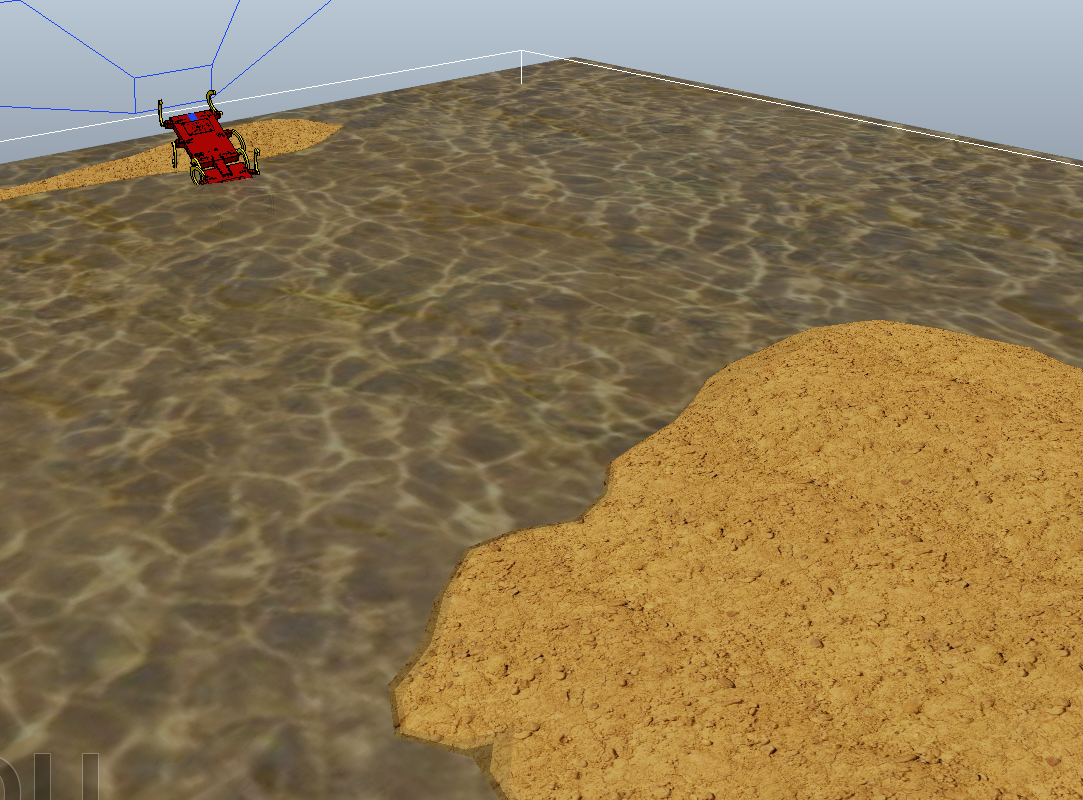
\includegraphics[height=5cm,width=1\textwidth,keepaspectratio]{terrain_w_water_end.png}
            \caption*{Конец маршрута}
        \end{subfigure}
        \begin{subfigure}[t]{0.26\textwidth}
            \centering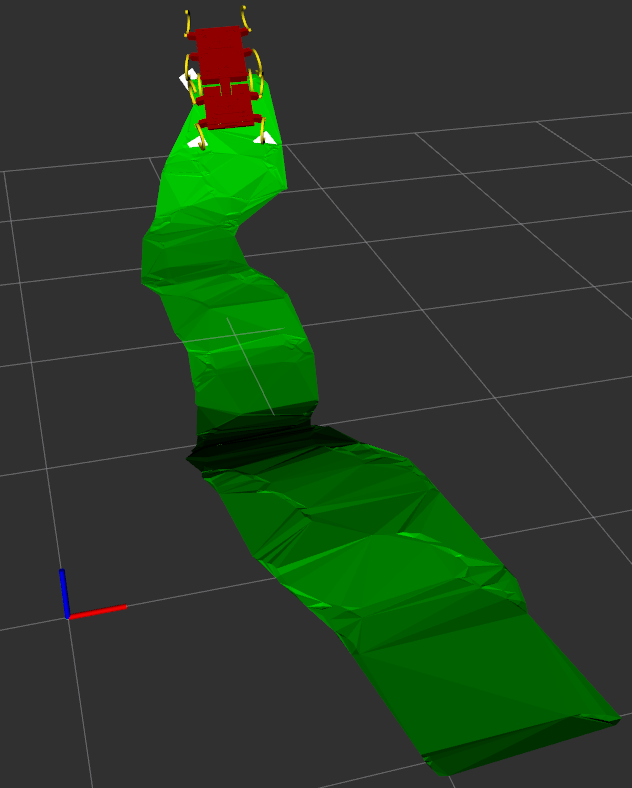
\includegraphics[height=5cm,width=1\textwidth,keepaspectratio]{mesh_rviz.png}
            \caption*{Созданная сетка}
        \end{subfigure}
    \end{figure}
\end{frame}

\note{d}

\begin{frame}[t]{Определение геометрических свойств поверхности}
    \framesubtitle{Результаты Cloud2Cloud и Cloud2Mesh}
    \begin{figure}[H]
        \begin{subfigure}[t]{0.49\textwidth}
            \centering\includegraphics[height=2.8cm,width=1\textwidth,keepaspectratio,page=10]{./tikz_pictures.pdf}
            % \caption*{Наложенные облака точек}
        \end{subfigure}
        \begin{subfigure}[t]{0.49\textwidth}
            \centering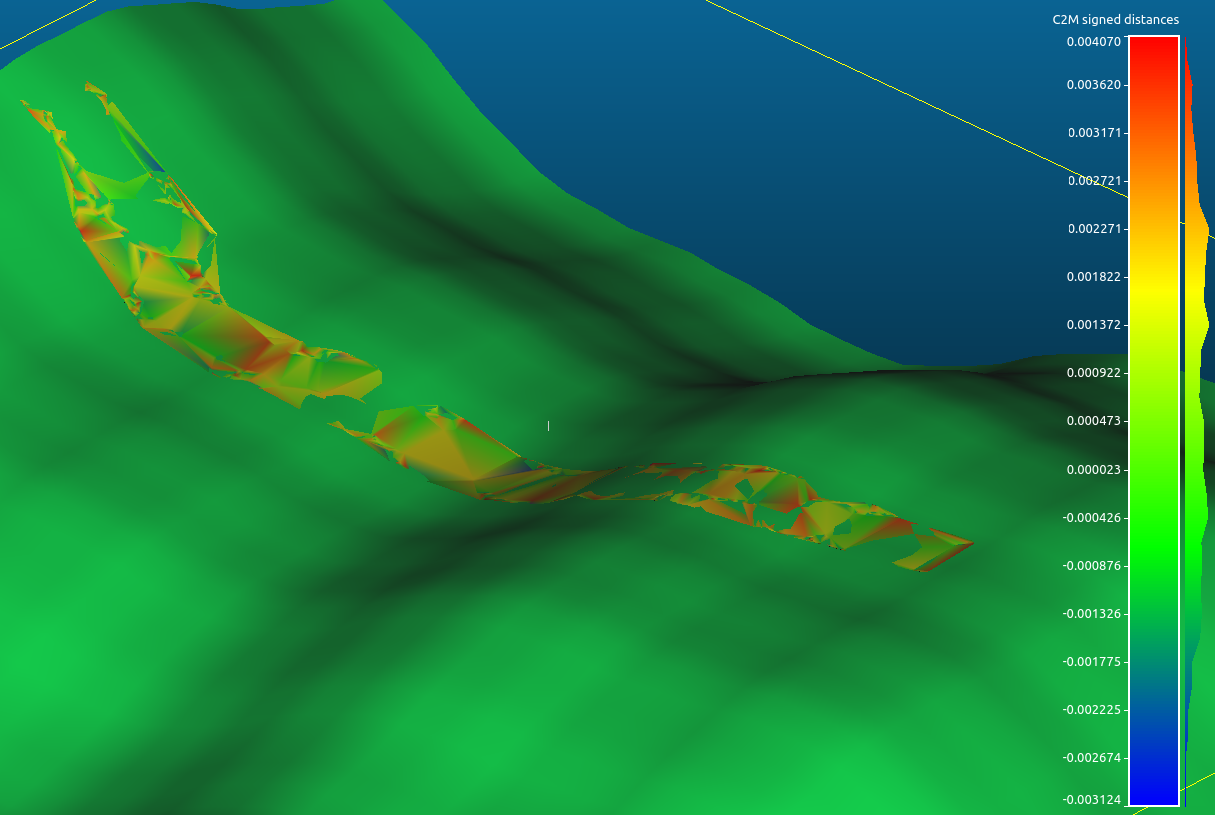
\includegraphics[height=2.8cm,width=1\textwidth,keepaspectratio]{mesh_comp.png}
            % \caption*{Наложенные сетки}
        \end{subfigure}

        \begin{subfigure}[t]{0.49\textwidth}
            \centering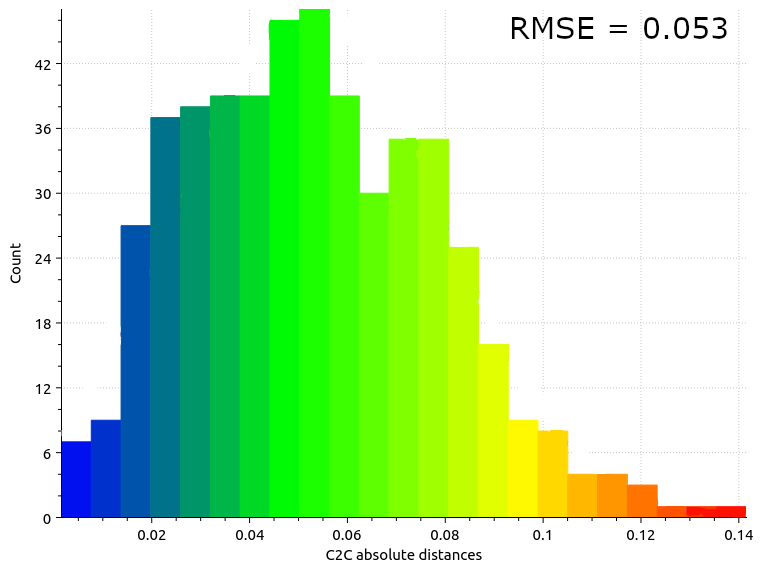
\includegraphics[height=2.6cm,width=1\textwidth,keepaspectratio]{pcd_hist.png}
            \caption*{Гистограмма ошибок C2C}
        \end{subfigure}
        \begin{subfigure}[t]{0.49\textwidth}
            \centering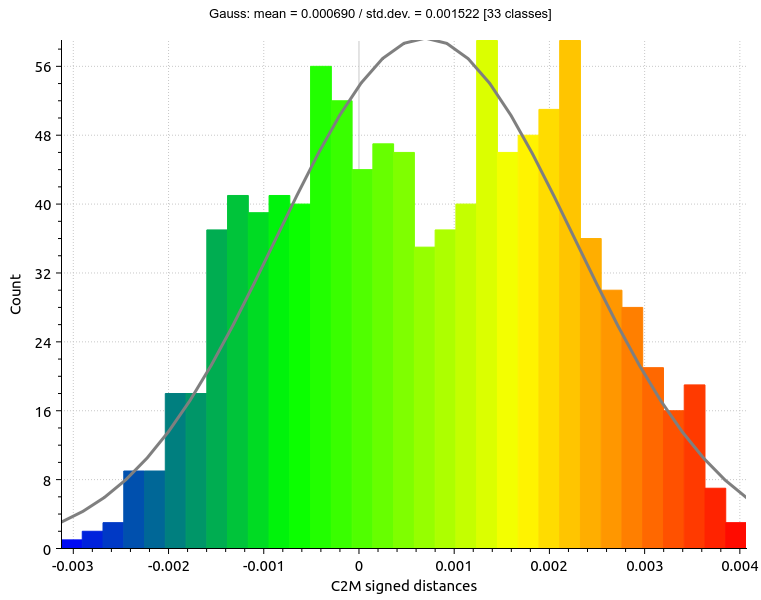
\includegraphics[height=2.6cm,width=1\textwidth,keepaspectratio]{mesh_hist.png}
            \caption*{Гистограмма ошибок C2M}
        \end{subfigure}
    \end{figure}
\end{frame}

\note{m}

\begin{frame}[t]{Определение геометрических свойств поверхности}
    \framesubtitle{Результат: Натурные испытания, Видео}
    \vspace{-0.5cm}
    \begin{figure}[H]
        \begin{subfigure}[t]{0.49\textwidth}
            % \href{run:./videos/big_angle2.mp4}{
            \href{https://youtu.be/2dxHHTG4psQ}{
                \centering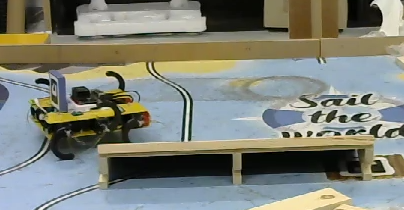
\includegraphics[height=6cm,width=1\textwidth,keepaspectratio]{real_robot_mesh_video_preview.png}}
            \caption*{Робот проходит препятствие}
        \end{subfigure}
        \begin{subfigure}[t]{0.49\textwidth}
            \centering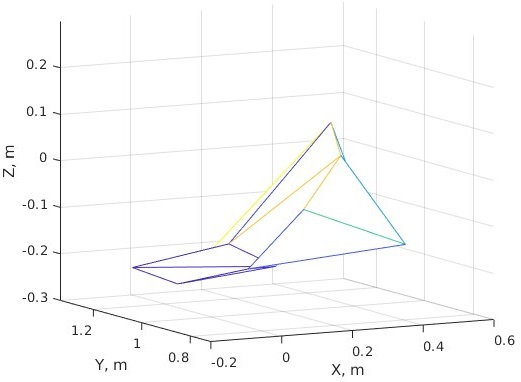
\includegraphics[height=6cm,width=1\textwidth,keepaspectratio]{real_mesh.jpg}
            \caption*{Полигональная сетка, полученная с помощью ног}
        \end{subfigure}
    \end{figure}
\end{frame}

\note{k}